\newif\ifonecolumn % Boolean to keep track of column mode (can use to format formulas etc)
%\documentclass{IEEEtran}\onecolumnfalse
%\documentclass[12pm,draftcls,onecolumn]{IEEEtran}\onecolumntrue

% ------------------------------------------------------------------------------
%   New IEEE Transactions Color Template
\documentclass[journal,twoside,web]{ieeecolor}\onecolumnfalse
% \documentclass[journal,twoside,web,onecolumn]{ieeecolor}\onecolumntrue
%\documentclass[journal,twoside,web,onecolumn]{ieeecolor}\onecolumntrue
%\documentclass[journal,12pt,onecolumn,draftclsnofoot,]{ieeecolor}

\usepackage{generic}
% \usepackage{cite}
% \def\BibTeX{{\rm B\kern-.05em{\sc i\kern-.025em b}\kern-.08em
%     T\kern-.1667em\lower.7ex\hbox{E}\kern-.125emX}}
% \markboth{\journalname, VOL. XX, NO. XX, XXXX 2018}
% {Author \MakeLowercase{\textit{et al.}}: Preparation of Papers for IEEE TRANSACTIONS and JOURNALS (February 2017)}
% ------------------------------------------------------------------------------

\pdfoutput=1
\pdfminorversion = 4

      
% !TEX root = main_min_disc_dist.tex
\usepackage{amsmath}
\usepackage{amsfonts}
%\usepackage{amsthm}
\usepackage{bm}
\usepackage{mathabx}
\usepackage[ruled,vlined,titlenotnumbered]{algorithm2e} 
\usepackage{graphicx} 
\usepackage{subcaption}
\usepackage{epsfig} 
\usepackage{cancel}
\usepackage{amssymb}
\usepackage{color}
\usepackage{resizegather} 
\usepackage{amssymb}


\usepackage{todonotes}
\newcommand{\smalltodo}{\todo[size=\footnotesize]}
\newcommand{\linetodo}{\todo[inline]}
\setlength{\marginparwidth}{1.3cm}


\usepackage{ifthen}
\newboolean{include-notes}
\setboolean{include-notes}{true}
 \newcommand{\jfnote}[1]{\ifthenelse{\boolean{include-notes}}%
 {\textcolor{blue}{\textbf{[JF: #1]}}}{}}

\usepackage{enumerate}

\usepackage{url}
\usepackage{hyperref}
\usepackage[%
   style=ieee,
   sorting=nyt,
   backend=bibtex,
   sortcites=true,
   doi=false,
   firstinits=true,
   hyperref,
   isbn=false,
   eprint=false,
   maxcitenames=3,
   block=none]
   {biblatex}
   
   \renewbibmacro{in:}{}
   \AtEveryBibitem{
 	\clearlist{language}
	\clearfield{pages}
	\clearfield{number}
	\clearfield{volume}
	}

\DeclareBibliographyCategory{needsurl}
\newcommand{\entryneedsurl}[1]{\addtocategory{needsurl}{#1}}
\renewbibmacro*{url+urldate}{%
 \ifcategory{needsurl}{
   \printfield{url}%
   \iffieldundef{urlyear}
     {}
     {\setunit*{\addspace}%
      \printurldate}}
   {}}

\renewcommand*{\bibfont}{\small}





\newcommand{\A}{\mathcal{A}}
\newcommand{\B}{\mathcal{B}}
\newcommand{\C}{\mathcal{C}}
\newcommand{\D}{\mathcal{D}}
\newcommand{\E}{\mathcal{E}}
\newcommand{\F}{\mathcal{F}}
\newcommand{\G}{\mathcal{G}}
\renewcommand{\H}{\mathcal{H}}
\newcommand{\I}{\mathcal{I}}
\newcommand{\J}{\mathcal{J}}
\newcommand{\K}{\mathcal{K}}
\renewcommand{\L}{\mathcal{L}}
\newcommand{\M}{\mathcal{M}}
\newcommand{\N}{\mathcal{N}}
\renewcommand{\O}{\mathcal{O}}
\renewcommand{\P}{\mathcal{P}}
\newcommand{\Q}{\mathcal{Q}}
\newcommand{\R}{\mathcal{R}}
\renewcommand{\S}{\mathcal{S}}
\newcommand{\T}{\mathcal{T}}
\newcommand{\U}{\mathcal{U}}
\newcommand{\V}{\mathcal{V}}
\newcommand{\W}{\mathcal{W}}
\newcommand{\X}{\mathcal{X}}
\newcommand{\Y}{\mathcal{Y}}
\newcommand{\Z}{\mathcal{Z}}


\renewcommand{\AA}{\mathbb{A}}
\newcommand{\BB}{\mathbb{B}}
\newcommand{\CC}{\mathbb{C}}
\newcommand{\DD}{\mathbb{D}}
\newcommand{\EE}{\mathbb{E}}
\newcommand{\FF}{\mathbb{F}}
\newcommand{\GG}{\mathbb{G}}
\newcommand{\HH}{\mathbb{H}}
\newcommand{\II}{\mathbb{I}}
\newcommand{\JJ}{\mathbb{J}}
\newcommand{\KK}{\mathbb{K}}
\newcommand{\LL}{\mathbb{L}}
\newcommand{\MM}{\mathbb{M}}
\newcommand{\NN}{\mathbb{N}}
\newcommand{\OO}{\mathbb{O}}
\newcommand{\PP}{\mathbb{P}}
\newcommand{\QQ}{\mathbb{Q}}
\newcommand{\RR}{\mathbb{R}}
\renewcommand{\SS}{\mathbb{S}}
\newcommand{\TT}{\mathbb{T}}
\newcommand{\UU}{\mathbb{U}}
\newcommand{\VV}{\mathbb{V}}
\newcommand{\WW}{\mathbb{W}}
\newcommand{\XX}{\mathbb{X}}
\newcommand{\YY}{\mathbb{Y}}
\newcommand{\ZZ}{\mathbb{Z}}

\newcommand{\fixwidth}[1]{\resizebox{\columnwidth}{!}{\ensuremath{\displaystyle{#1}}}} 


\newcommand{\Dx}{\hat\D(x)}
\newcommand{\XXD}{\XX_{\hat{\D}}}
\newcommand{\bu}{\bm{u}}
\newcommand{\bdelta}{\bm{d}}
\newcommand{\bgamma}{\bm{\gamma}}
\newcommand{\bbeta}{\bm{\beta}}
\newcommand{\bphi}{\bm{\phi}}
\newcommand{\bx}{\xi}

\newcommand{\Disc}{\text{Disc}}
\DeclareMathOperator{\interior}{int}

\newcommand{\optud}{\underset{u\in\U}{\max}\text{ }\underset{ d\in\D}{\min}}
\newtheorem{claim}{Claim}
\newtheorem{definition}{Definition}
\newtheorem{theorem}{Theorem}
\newtheorem{lemma}{Lemma}
\newtheorem{corollary}{Corollary}
\newtheorem{remark}{Remark}
\newtheorem{proposition}{Proposition}
\newtheorem{assumption}{Assumption}


\newcommand{\Vsdr}{V_2}

\newenvironment{for_journal}{\par\color{black}}{\par}

\newenvironment{needs_work}{\par\color{red}}{\par}

\newcommand{\specialcell}[2][c]{%
  \begin{tabular}[c]{@{}l@{}}#2\end{tabular}}

% \bibliographystyle{ieeetr}
\bibliography{library}


\title{\LARGE \bf
A Minimum Discounted Reward Hamilton-Jacobi Formulation for Computing Reachable Sets 
}
\author{
Anayo K. Akametalu\textsuperscript{1}, \and Shromona Ghosh\textsuperscript{1}, \and Jaime F. Fisac\textsuperscript{1}, and \and Claire J. Tomlin\textsuperscript{1}
\thanks{
\textsuperscript{1}Department of Electrical Engineering and Computer Sciences, 
        University of California, Berkeley. Cory Hall, Berkeley, CA 94720, United States.\newline
        {\tt\small \{kakametalu, shromona.ghosh, jfisac, tomlin\}~@eecs.berkeley.edu }}% 
\thanks{
This work is supported by NSF under the CPS FORCES and VehiCal projects, by the UC-Philippine-California Advanced Research Institute, and the ONR MURI Embedded Humans. It is also supported through the Army Research Laboratory and was accomplished under Cooperative Agreement Number W911NF-17-2-0196; and in part by Toyota under the iCyPhy center. The research of A.K. Akametalu has received funding from the National GEM Consortium Fellowship.} 
}
%TODO: Do we want to reincorporate the 
%
\begin{document}
\maketitle
\thispagestyle{empty}
\pagestyle{empty}

\begin{abstract}
We propose a novel formulation for approximating reachable sets through a minimum discounted reward optimal control problem. The formulation yields a continuous solution that can be obtained by solving a Hamilton-Jacobi equation. Furthermore, the numerical approximation to this solution can be obtained as the unique fixed-point to a contraction mapping. This allows for more efficient solution methods that could not be applied under traditional formulations for solving reachable sets. In addition, this formulation provides a link between reinforcement learning and learning reachable sets for systems with unknown dynamics, allowing algorithms from the former to be applied to the latter. We use two benchmark examples, double integrator, and pursuit-evasion games, to show the correctness of the formulation as well as its strengths in comparison to previous work.
\end{abstract}


\section{Introduction \label{sec:intro}}
% !TEX root = main_min_disc_dist.tex

Computing reachable sets has been a popular approach for verifying and validating the behavior of dynamical systems. In the reachability problem, one specifies a target set in the state space and then aims to find the set of initial states admitting trajectories that can eventually enter the target within some specified time horizon. The target may represent a region we desire to drive the system to or keep the system away from. Due to its generality, Hamilton-Jacobi (HJ) reachability analysis, which casts the problem in the optimal control framework, has seen broad usage in many safety-critical applications including emergency landing of unmanned aerial vehicles (UAVs) \cite{Ding2016}, vehicle platooning \cite{Chen2015a}, safe learning \cite{Akametalu2014, Gillula2012}, collision-avoidance \cite{Hoffmann2008, Mitchell2005}, and many others \cite{Ding2011a, Huang2011}.


The standard HJ formulation for reachability solves a \emph{minimum reward} (MR) optimal control problem, by computing the viscosity solution of a particular time-dependent HJ partial differential equation (PDE) \cite{Mitchell2005}. Like most optimal control problems the solution is solved approximately on a grid via value iteration, which recursively applies a \emph{backup operator} until convergence. One downside of MR optimal control problems is that the backup operator in this setting is not a contraction mapping, thus a specific initialization of value iteration is required for convergence to the correct solution. A contraction mapping allows for arbitrary initialization, and with a good initialization convergence can be accelerated. This is particularly useful when computing reachable sets for multiple systems with similar dynamics allowing for the solution of one problem to be used as an initialization for the other.

On the other hand, infinite horizon \emph{sum of discounted reward} (SDR) problems yield backup operators that are contraction mappings \cite{Bertsekas1995}. This allows for more efficient solution methods, like policy iteration \cite{Howard1964, Puterman1979} and multigrid approaches \cite{Alla2015, Chow1991}.   
 
Drawing inspiration from SDR problems, we propose a \emph{minimum discounted reward} (MDR) formulation for computing tight over- and under-approximations of infinite horizon reachable sets. This new formulation yields a contraction mapping, making it possible to extend policy iteration and multigrid approaches to this setting. In addition, it also provides a way forward for learning reachable sets when dynamics are unknown or difficult to model, a topic that has garnered some attention recently \cite{Akametalu2015,Djeridane2006}. This draws greatly from Reinforcement Learning (RL), which attempts to solve the infinite horizon SDR problem when the system model is unknown. Many RL algorithms boil down to finding the fixed-point of the backup operator associated with SDR. The techniques developed in RL, like temporal differencing \cite{Sutton1988} and Q-learning \cite{Watkins1992}, can naturally be extended to do the same in the MDR setting, thus facilitating research in learning reachable sets.

The paper is organized as follows in Section \ref{sec:back} we briefly go over the MR formulation for HJ reachability analysis, and SDR problems. In Section \ref{sec:mdr} we describe the minimum discounted  reward formulation, and prove some relevant results. In Section \ref{sec:conv} we explore policy iteration and multigrid approaches within the context of the MDR. Section \ref{sec:learn}draws inspiration from RL and presents some preliminary ideas on how the formulation can be used for learning reachable sets. Section \ref{sec:sim} contains examples demonstrating the ideas developed throughout the paper, and we conclude the paper in Section \ref{sec:end}.

\subsection*{Terminology}

The term \emph{optimal control} is typically reserved for the one-player setting, and \emph{differential game} is used when considering problems with two or more players. Here, both the one-player and two-player settings are considered, and we opt to use the terminology from optimal control for consistency. For example \emph{optimal control} will be used to refer to both settings, and we use terms like \emph{reward} instead of \emph{payoff} throughout.

% Computing reachable sets have been a popular approach for verifying and validating the behavior of dynamical systems. In most applications, practitioners specify a target set in the state space and then aim to find the set of initial states admitting trajectories that can eventually enter the target within some specified time horizon, i.e. the \emph{backward reachable set}. The reachable set can be used to provide guarantees on the liveness of the system if the goal is to enter the target set, e.g. finding the basin of attraction for a reference point. It can also be used for safety applications, where the target set represents unsafe states and the reachable set thus represents states that are potentially unsafe, e.g. collision avoidance.

% One of the most general approaches for computing reachable sets is through Hamilton-Jacobi (HJ) reachability analysis which has its theoretical underpinnings in optimal control and differential games. The approach can handle non-linear dynamics, and only requires that the target set be closed.  Other methods restrict the target to either hyperplanes or ellipsoids \cite{Frehse2011, Greenstreet1998, Kurzhanski2000}. Due to its generality HJ reachability analysis has been used in a number of safety-critical applications including emergency landing of unmanned aerial vehicles (UAVs) \cite{Ding2016}, vehicle platooning \cite{Chen2015a}, safe learning \cite{Akametalu2014, Gillula2012}, collision-avoidance \cite{Hoffmann2008, Mitchell2005}, and many others \cite{Ding2011a, Huang2011}. 

% The reachable sets can be constructed either through a \emph{minimum distance} (also referred to as time-dependent) or \emph{minimum time to reach} (also referred to as time-independent) HJ formulation. In the minimum distance formulation the viscosity solution to a particular time-dependent HJ partial differential equation (PDE) is shown to be an implicit surface representation of the backwards reachable set \cite{Mitchell2005}. This same viscosity solution is also obtained by solving a particular time-dependent HJ variational inequality (VI) \cite{Barron1989, Barron1990}. The solution represents the \emph{minimum distance function}, i.e. for any given initial state and time horizon the minimum distance to the target set the system will realize along an optimal trajectory. \footnote{The term distance here is user defined and quite general. The only requirement is that the distance function is continuous, negative inside the target set, and nonnegative otherwise. Optimality of the trajectory depends on whether the objective is to enter the target or avoid the target.} The minimum time to reach formulation obtains the minimum time to reach function as a solution to a time-independent HJI PDE  \cite{Bardi1999, Falcone1994}. The reachable sets are then just super-zero level sets of the time to reach function. 

% The authors of \cite{Mitchell2005} state some advantages for using the minimum distance formulation. The most important advantage is that the minimum distance function is continuous, and thus numerically easier to handle than the minimum time to reach function which can have discontinuities. Finally, the time to reach formulation is not well-defined outside the reachable set, thus it provides no information on constructing control laws to avoid the reachable set in safety applications. The minimum distance formulation does not have this limitation.

% This paper is focused on the infinite horizon reachable set, which is relevant for scenarios where the system may be in operation for long periods of time, e.g. reinforcement learning or vehicle platooning. In the infinite horizon context the minimum time to reach formulation has a key advantage over the minimum distance formulation. In both approaches the solutions are approximated on a grid, and iteratively solved until convergence via dynamic programming (DP). The minimum distance formulation is only guaranteed to converge to the correct result if the DP algorithm is initialized with the distance function. On the other hand, the minimum time to reach formulation is agnostic to the initialization. A key insight here is if a good approximation to the solution is used as an initialization, then the DP algorithm will have faster convergence. This is the underlying idea behind policy iteration and multi grid approaches, which both try to obtain good approximations cheaply and often times perform better than the standard DP algorithm.

% Since the minimum time to reach function is unbounded (for states that never reach the target), it is actually solved as an infinite horizon sum of discounted rewards problem through the Kruzkhov transform \cite{Falcone2014}. Discounting induces a DP algorithm that acts as a contraction mapping with a unique fixed point.

% In this paper we propose a discounted minimum distance formulation that both yields a solution that is continuous, and a DP algorithm that acts as a contraction mapping with a unique fixed point. Implicit surface representations of over and under approximations of the reachable set can be obtained from the solution. The error in the approximations can be controlled by the amount of discounting introduced, which also impacts the convergence properties of the DP algorithm. 

% The paper is organized as follows in Section \textcolor{red}{Blah} we briefly go over the minimum distance formulation for HJI reachability analysis, and sum of discounted reward problems. In Section \textcolor{red}{Blah} we describe the discounted minimum distance formulation, and prove some relevant results (continuity of the solution, DP algorithm is a contraction mapping, etc.). In Section \textcolor{red}{Blah} we present some ideas for producing good approximations for improved convergence, which include policy iteration and multigrid approaches. Section \textcolor{red}{Blah} draws inspiration from Reinforcement Learning and presents some preliminary ideas on how the formulation can be used for learning the reachable set when the system model is not known or cannot be written down explicitly. Section \textcolor{red}{Blah} contains examples demonstrating the ideas developed throughout the paper, and finally we close with our conclusion in Section \textcolor{red}{Blah}.


\section{Background \label{sec:back}} 
% !TEX root = main_min_disc_dist.tex

We consider a two-player optimal control problem where the first player (control) wants to keep the system away from the target set for a given time horizon and the second player (disturbance) has the opposite objective.\footnote{We can also consider the case where the objectives are switched, and the control wants to drive the system towards the target, by making minor modifications to the material presented here.} Our goal is to characterize the \emph{infinite-horizon backward reachable set}, which is the set of initial states for which the disturbance wins the game. Going forward all mentions of reachable set refer to the infinite horizon backwards reachable set.

\subsection{System Model \label{subsec:dynamics}}

The analysis in this paper considers a fully observable system whose underlying dynamics may be non-deterministic, but bounded. 
We can formalize this as a dynamical system with state $x\in\RR^n$, and two inputs, $u\in\U\subset\RR^{n_u},  d\in\D\subset\RR^{n_d}$
(with $\U$ and $\D$ compact)
which we will refer to as the \emph{controller} and the \emph{disturbance}:
\begin{equation}\label{fxud}
\dot{x} = f(x,u, d).
\end{equation}

The flow field $f: \RR^n \times \U \times \D\rightarrow\RR^n$ is assumed to be Lipschitz continuous and bounded. In the single-player case we drop the disturbance input, and just have ${f(x,u):\RR^n \times \U \rightarrow\RR^n}$.

Letting $\UU $ and $\DD$ denote the collections of measurable%
	\footnote{A function $f:X\to Y$ between two measurable spaces $(X,\Sigma_X)$ and $(Y,\Sigma_Y)$
	is said to be measurable if the preimage of a measurable set in $Y$ is a measurable set in $X$, that is:
	$\forall V\in\Sigma_Y, f^{-1}(V)\in\Sigma_X$, with $\Sigma_X,\Sigma_Y$ $\sigma$-algebras on $X$,$Y$.}
functions $\bm u: [0,\infty)\to \U $ and $\bm d: [0,\infty)\to \D$ respectively,
and allowing the controller and disturbance to choose any such signals,
the evolution of the system
from any initial state $x$
is determined (see for example \cite{Coddington1955}, Ch.~2, Theorems~1.1,~2.1) by the unique continuous trajectory $\bx:[0,\infty)\to\RR^n$ solving
\begin{equation}\label{eq:xdot}
\begin{split}
\dot{\bx}(s) &= f(\bx(s),\bu(s),\bdelta(s)), \text{ a.e. }s\ge 0,\\
\bx(0) &= x.
\end{split}
\end{equation}
Note that this is a solution in Carath\'eodory's \emph{extended sense}, that is, it satisfies the differential equation \emph{almost everywhere} (i.e. except on a subset of Lebesgue measure zero).


Throughout our analysis, we will use the notation $\bx_{x}^{\bu,\bdelta}(\cdot)$ to denote the state trajectory $t\mapsto x$ corresponding to the initial condition $x\in\RR^n$, the control signal $\bu\in\UU$ and the disturbance signal $\bdelta\in\DD$.


\subsection{HJ Reachability: Minimum Distance to Target}
The target set $\T$ can be implicitly characterized as the sub-zero level set of a Lipschitz \emph{surface function} $l:\RR^n\rightarrow\RR$: 
\begin{equation}\label{eq:l}
x\in\T\iff l(x)<0.
\end{equation}
This function always exists, since we can simply choose the \emph{signed distance function} to $\T$,  $s_{\T}(x)$, which is Lipschitz continuous by construction.\footnote{ For any nonempty set $\M\subset\RR^m$, the signed distance function $s_{\M}:\RR^m\to\RR$  is defined as
$\inf_{y\in\M} |z-y|$ for points outside of $\M$ and $ -\inf_{y\in\RR^m\setminus\M} |z-y|$ for points inside $\M$, where $|\cdot|$ denotes a norm on $\RR^m$.} We use a clipped signed distance since the problem is solved over a fixed domain in practice, $l(x) = \min(\max(s_{\T}(x), -L), L)$ with $L>0$, where $L$ is usually taken to be the largest value (in magnitude) on the domain.

To express whether a given trajectory \emph{ever} enters the target set, let the functional $\V:\RR^n\times\UU\times\DD\to\RR$ assign to each initial state $x$ and input signals $\bu(\cdot)$, $\bdelta(\cdot)$ the lowest value of $l(\cdot)$ achieved by trajectory $\bx_{x}^{\bu, \bdelta}(\cdot)$ over all times $t\ge0$: 
\begin{equation}\label{eq:min_dist_functional}
\mathcal{V}\big(x,\bu(\cdot),\bdelta(\cdot)\big) := \inf_{t\ge 0}l\big(\bx_{x}^{\bu,\bdelta}(t)\big).
\end{equation}
This outcome $\V$, also referred to here as the \emph{minimum of rewards}\footnote{In this context reward refers to $l(x)$, but in general it can be any real-valued function.}, will be nonpositive if there exists any $t\in[0,\infty)$ at which the trajectory enters the target set, and will be strictly positive if the system avoids the target for all $t\ge 0$. 

% Denoting $\V^{\bu,\bdelta}(x) = \V\big(x,\bu(\cdot),\bdelta(\cdot)\big)$, the following statement follows from \eqref{eq:l} and \eqref{eq:min_dist_functional} by construction. 

% \begin{proposition}\label{Value}
% The set of points $x$ from which the system trajectory $\bx^{\bu,\bdelta}_{x}(\cdot)$ under given inputs $\bu(\cdot)\in\UU,\bdelta(\cdot)\in\DD$ will enter the target set $\T$ for some time $t\ge0$ is equal to the zero sublevel set of $\mathcal{V}^{\bu,\bdelta}(\cdot)$:
% \[
% \{x\in\RR^n: \exists t\ge0,\; \bx^{\bu,\bdelta}_{x}(t)\in\T\}=\{x\in\RR^n: \mathcal{V}^{\bu,\bdelta}(\cdot)\le0\}.
% \]
% \end{proposition}


The reachable set can then be obtained by solving a game between the controller and disturbance where the disturbance can use \emph{nonanticipative strategies} to respond to the controller's signal. The disturbance's set of nonanticipative strategies is $\B = \{\bbeta:\UU\to\DD\;|\;
\forall t\ge 0,\; \forall \bu(\cdot),\hat{\bu}(\cdot)\in\UU,$
${\big(\bu(\tau) \!=\! \hat{\bu}(\tau)\text{ a.e.} \tau\ge0\big)\Rightarrow
{\big(\bbeta[\bu](\tau) \!=\! \bbeta[\hat{\bu}](\tau)}{\text{ a.e.} \tau\ge0\big)}}\}$. Intuitively, the disturbance is given an instantaneous informational advantage in the game, but its actions at any given time can only depend on what the controller has done up to that time. With this in place we can define the \emph{value function} $V(x)$ and ultimately the reachable set $\R(\T)$. 
%
\begin{equation} \label{eq:val_function}
V(x)=\inf_{\beta[\bu](\cdot) \in \B} \sup_{\bu \in \UU}\mathcal{V}\big(x,\bu(\cdot),\beta[\bu](\cdot)\big),
\end{equation}
%
\begin{equation} \label{eq:reach_set}
\R(\T) = \{x \mid V(x) \le 0\}.
\end{equation}  

The optimization in \eqref{eq:val_function} is referred to here as the minimum reward optimal control problem. It has been shown that the value function for problems with outcome given by equation \eqref{eq:min_dist_functional} can be characterized as the unique viscosity solution to a variational inequality \cite{Barron1990}. When the problem is solved over a finite time interval $[0,T]$, the \emph{finite-horizon value function} $V(x,t)$ can be computed by solving the HJ equation: 
%
\begin{equation} \label{eq:HJ_mr}
\begin{split} 
    & 0 = \min\left\{l(x)-V(x,t), \frac{\partial V}{\partial t}(x,t)+ \max_{u\in\U} \min_{ d\in\D} \!\!\frac{\partial V}{\partial x}(x,t) f(x,u, d)\right\}\\
    &V(x,T) = l(x).
\end{split}
\end{equation}
%
 As $T \rightarrow \infty$, $V(x,t)$ becomes independent of $t$. We accordingly drop the dependence on $t$ and recover $V(x)$ as defined in \eqref{eq:val_function}. 


\subsection{Computing the Value Function}
Several approximation schemes have been proposed for solving \eqref{eq:HJ_mr} and similar HJ equations on a fixed grid $G$ \cite{Bardi1999, Falcone1994, Mitchell2005}. Here we will use a semi-Lagrangian approximation based on a discrete time dynamic programming (DP) principle:
%
\begin{subequations}
\begin{align}
&V_{\Delta t}^{k+1}(x) = \min\{l(x),  \underset{u\in\U}{\max}\text{ }\underset{ d\in\D}{\min} V^{k}_{\Delta t}(x+\Delta t f(x,u,d))\}\\
&V_{\Delta t}^{0}(x) = l(x)\\
&V_{\Delta t} = \lim_{k\rightarrow \infty} V^{k}_{\Delta t},
\end{align}
\end{subequations}%
\noindent where $V_{\Delta t}(x)$ converges to $V(x)$ as the discrete time step $\Delta t \rightarrow 0$. With the semi-Lagrangian approximation, the value function is solved on a discrete grid. Representing the approximation in vectorized form, $\vec{V} \in \RR^{N_G}$, the semi-Lagrangian approach yields \ 
\begin{subequations} \label{eq:dp_min_dist}
\begin{align}
&\vec{V}_{i}^{0} = l(x_i)\\
&\vec{V}_{i}^{k+1} = \min\{l(x_i),  \underset{u\in\U}{\max}\text{ }\underset{ d\in\D}{\min} I[\vec{V}^{k}](x_i+\Delta t f(x_i,u,d)) \label{eq:dp_min_dist_b}\}\\
&\vec{V} = \lim_{k\rightarrow \infty} \vec{V}^{k},
\end{align}
\end{subequations}%
\noindent for  $i=1, ..., N_G$, where $\{x_i\}_{i=1}^{N_G}$ are the grid nodes, $N_G$ is the number of grid nodes, $\vec{V}_i^k$ is the approximate value for $V(x_i, k \Delta t)$ and ${I[\vec{A}]:\RR^n \rightarrow \RR}$ represents an interpolation operator defining, for every point $x$, the polynomial reconstruction based on the values $\vec{A}$. Unless stated otherwise $G$ is taken to be a regular equidistant array of points with mesh spacing $\Delta x_j$ along the $j$th axis, $j=1,...,n$.\footnote{In the most general case the control and disturbance sets are also discretized, $\U=\{u_i\}_{i=1}^{N_U}$ and $\D=\{d_i\}_{i=1}^{N_D}$, and the minimax game is approximated.} We use a multilinear interpolator is used for the interpolation scheme, thus the interpolation function $I[\vec{A}](\cdot)$ is given by a convex combination over the elements of $\vec{A}$,
\begin{equation}
I[\vec{A}](x)= p(x)\cdot \vec{A},
\end{equation}%
\noindent where the elements of ${p(\cdot): \RR \rightarrow \RR^{N_G}}$ are greater than zero and sum to one. 

For conciseness we introduce \emph{control policies} ${\pi_u(\cdot): \RR^n \rightarrow \U}$ and \emph{disturbance policies} ${\pi_d(\cdot): \RR^n \rightarrow \D}$, which map from state to control and state to disturbance, respectively. Note that the individual minimax games being played at each grid point can be collectively thought of as a game over policies. We also introduce the \emph{backup operator} ${B[\cdot]: \RR^{N_G} \rightarrow \RR^{N_G}}$, which maps vectorized value functions onto themselves. Define the backup operator as
%
\begin{equation} \label{eq: op_min_dist}
 B[\vec{A}] := \min\{\vec{l},  \underset{\pi_u}{\max}\text{ }\underset{ \pi_d}{\min} P_{\pi_u, \pi_d} \vec{A}\},
\end{equation}%
\noindent where ${\vec{l} \in \RR^{N_G}}$ with ${\vec{l}_i = l(x_i)}$ for ${i=1, ..., N_G}$, ${P_{\pi_u, \pi_d} \in \RR^{N_G \times N_G}}$ is a policy-dependent stochastic matrix\footnote{$P_{\pi_u, \pi_d}$ is effectively the probability transition matrix for a Markov Decision Process (MDP) over a finite state space given by the grid nodes ${\{x_i\}_{i=1}^{N_G}}$.}, and row $i$of $P_{\pi_u, \pi_d}$ is $p(x_i+\Delta tf(x, \pi_u(x_i), \pi_d(x_i)))$. For the one player setting this matrix becomes $P_{\pi_u}$. We can now express \eqref{eq:dp_min_dist} more concisely as
%
\begin{subequations}\label{eq:val_iter}
\begin{align}
&\vec{V}^{0} = \vec{l}\\
&\vec{V}_{i}^{k+1} = B[V^k] \\
&\vec{V} = \lim_{k\rightarrow \infty} \vec{V}^{k}.
\end{align}
\end{subequations}

This recursive procedure \eqref{eq:val_iter} is referred to as \emph{value iteration}, and here $\vec{V}$ is the \emph{vectorized value function}, which is used to approximate the value function $V(x)$ as $I[\vec{V}](x)$. 

The value iteration algorithm in \eqref{eq:val_iter} can be used to solve other optimal control problems, albeit with a different backup operator and initialization $\vec{V}^{0}$. As other optimal control problems are presented we redefine the backup operator and specify the initialization required for the value iteration procedure.

\subsection{Contraction Mappings and Sum of Discounted Rewards}

Value iteration converges to a unique solution, independent of the initialization, when the backup operator is a \emph{contraction mapping}.  
%
\begin{definition} A mapping $M(\cdot): \RR^{N_G} \rightarrow \RR^{N_G}$, is said to be a contraction mapping in the norm $|| \cdot ||$ over the space $\RR^{N_G}$ if there exists a Lipschitz constant $0\leq \kappa < 1$ such that for any $\vec{A}_1, \vec{A}_2 \in \RR^{N_G}$, $||M(\vec{A}_1) - M(\vec{A}_2)|| \leq \kappa ||\vec{A}_1 - \vec{A}_2||$. 
\end{definition}

By the contraction mapping theorem any contraction mapping has a unique fixed point. The operator given by \eqref{eq: op_min_dist} is not a contraction mapping. To see this note that any vector $\alpha \vec{1} \in \RR^{N_G}$ is a fixed point for $\alpha < -L$.

The SDR problem does yield a contraction mapping, and we explore it briefly for the one player case. The objective is to maximize the integral (sum) of exponentially discounted rewards. In an abuse of notation, the associated value function $V(x)$ for this problem is given by
%
\begin{equation}\label{eq:V_sum_rewards}
V(x) := \sup_{\bu \in \UU} \int_{0}^{\infty}r\big(\bx_{x}^{\bu}(t)\big)\exp(-\lambda t) dt,  \quad \lambda >0,
\end{equation}%
\noindent where $r(\cdot):\RR^n \rightarrow \RR$ is a state-dependent reward function, and $\lambda$ is a \emph{discount factor}.

It is known that this value function is the solution to the time-independent Hamilton-Jacobi equation \cite{Bardi2008},
%
\begin{equation} \label{eq:HJ_sdr}
\lambda V(x) = \max_{u\in\U} \frac{\partial V}{\partial x}(x) f(x, u)+ g(x).
\end{equation}

Using the same semi-Lagrangian scheme as in the MR setting, equation \eqref{eq:HJ_sdr} can be approximated as
%
\begin{equation}
V_{\Delta t}(x) = \max_{u\in\U} \gamma V_{\Delta t}(x + \Delta t\cdot f(x, u))  + \Delta t \cdot r(x),
\end{equation}
 
\noindent where $\gamma=\exp(-\lambda \Delta t)$ is the \emph{discount rate}.

The approximation is solved for using value iteration with the following backup operator
%
\begin{equation} \label{eq:backup_sdr}
B[\vec{A}] := \vec{r} +  \underset{\pi_u}{\max} \gamma P_{\pi_u} \vec{A}, 
\end{equation}%
\noindent where $\vec{r}_i =\Delta t \cdot r(x_i)$. The initialization of the value iteration procedure is arbitrary $\vec{V}^{0} \in \RR^{N_G}$ because the backup  operator in \eqref{eq:backup_sdr} is a contraction mapping in the infinity norm, $||\cdot||_\infty$ \cite{Bertsekas1995}.

Discounting reduces the impact of future rewards on the outcome of the trajectory, and ultimately yields a contraction mapping. In fact, the discount factor $\gamma$ is the Lipschitz constant of the contraction mapping.


% \begin{needs_work}
%  The value function at any iteration can be thought of as an estimate of the impact of all future rewards, and the backup operator can be seen as combining these future rewards with the current reward $\vec{r}$. Essentially things that happen far into the future are ``forgotten", which includes errors in the initial estimate $\vec{V}^0$.  
% \end{needs_work}





\section{Minimum of Discounted Rewards \label{sec:mdr}}
% !TEX root = main_min_disc_dist.tex
Inspired by the SDR setting, we now present the MDR optimal control problem. Moving forward any mention of value function $V(x)$ refers to the MR setting, and is defined by \eqref{eq:min_dist_functional}, \eqref{eq:val_function}, and \eqref{eq:HJ_mr}.

\subsection{What to discount?}

A natural proposal for the outcome of the MDR problem would be
 
\begin{equation}
\inf_{t\ge 0}l\big(\bx_{x}^{\bu,\bdelta}(t)\big)\exp(-\lambda  t).
\end{equation}

However, there is an issue with defining this outcome. Recall that discounting makes rewards contribute less to the outcome the further they occur in the future. Since we take an infimum, the discounted reward should become more positive the further it occurs in the future making it less likely to be selected by the infimum. This only works if the reward is nonpositive everywhere, which is not the case for $l$, since it is a clipped signed distance. This is easily fixed with the following outcome for the MDR problem
%
\begin{equation}
\mathcal{Z}\big(x,\bu(\cdot),\bdelta(\cdot)\big) := L + \inf_{t\ge 0}(l\big(\bx_{x}^{\bu,\bdelta}(t)\big)-L)\exp(-\lambda  t).
\end{equation}%
\noindent The quantity in the infimum is always nonpositive since $L$ upperbounds $l(x)$ by construction. Note that if ${\lambda=0}$, i.e. no discounting, then we have the minimum reward outcome \eqref{eq:min_dist_functional}. 

We define the MDR value function as
%
\begin{equation} \label{eq:mdr_val_function}
Z(x):=\inf_{\beta[\bu](\cdot) \in \B} \sup_{\bu \in \UU}\mathcal{Z}\big(x,\bu(\cdot),\beta[\bu](\cdot)\big).
\end{equation}

For convenience we define two functions ${U(x):=Z(x)-L}$ and ${h(x):=l(x)-L}$. 
%
\begin{proposition}\label{prop:visc}
The function $U(x)$ is the unique viscosity solution to the following time-independent HJ equation
\begin{equation} \label{eq:HJ_mdr}
    0 = \min \left\{h(x)-U(x), \max_{u\in\U} \min_{ d\in\D} \!\!\frac{\partial U}{\partial x}(x) f(x,u, d) - \lambda U(x)\right\}.
\end{equation}
\end{proposition}%
\noindent Due to space constraints we omit the proof for Proposition \ref{prop:visc}, which follows the same structure as the viscosity proofs presented in \cite{Evans1984}. 

%Since $L$ is an additive constant, our attention can be focused on the payoff from the second term of equation (\ref{eq:V_lambda}), which yields a related value function
%
%\begin{equation}
%U_{\lambda}(x)=\inf_{\beta[\bu](\cdot) \in \B} \sup_{\bu \in \UU}\mathcal{V}_{\lambda}\big(x,\bu(\cdot),\bdelta(\cdot)\big)-L, 
%\end{equation}
%\noindent thus $V_{\lambda}(x) = U_{\lambda}(x)+L$. It can be shown that the above value function is the viscosity solution to the following variational equality


%% !TEX root = main_min_disc_dist.tex
\begin{for_journal}

For convenience we define two functions ${U(x):=Z(x)-L}$ and ${h(x):=l(x)-L}$. 
We will show that $U(x)$ is the viscosity solution to a particular time-independent HJ equation. We begin by presenting some Lemmas to facilitate the proof.
%
\begin{lemma}
The function $U(x)$ is well defined. 
\end{lemma} 
%
\begin{proof}
Define the sequence $\{U(x,k)\}_k$, where
%
\begin{equation}
U(x,k) = \inf_{\beta[\bu](\cdot) \in \B} \sup_{\bu \in \UU} \inf_{t \in [0,k\Delta t]}(h\big(\bx_{x}^{\bu,\beta[\bu]}(t)\big))\exp(-\lambda  t),
\end{equation}
%
and $\Delta t>0$. The sequence is nonincreasing, since $U(x,k+1) \leq U(x,k)$, and is lower bounded by $-2L$, so it converges. Clearly in the limit this sequence also equals $U(x)$.
\end{proof}



\begin{lemma} \label{dpp}
\emph{Dynamic programming principle.} For $\delta>0$,
%
\begin{equation}
\begin{split} 
U(x)= \inf_{\beta[\bu](\cdot) \in \B} \sup_{\bu \in \UU_\delta} 
\big [
\min\{&\inf_{t \in [0, \delta]} h\big(\bx_{x}^{\bu,\beta[\bu]}(t)\big))\exp(-\lambda  t), 
\\&\exp(-\lambda \delta)U(\bx_{x}^{\bu,\beta[\bu]}(\delta))\}
\big ]
\end{split},
\end{equation}
%
where $\UU_{\delta}$ consists of measurable functions on the interval
$[0,\delta]$.
\end{lemma}

\begin{proof}
Splitting the time interval of the infimum in \eqref{eq:mdr_functional} into $[0,\delta]$ and $t>\delta$, $U(x)$ can be expressed as
%
\begin{equation}
\begin{split}{}{}{}
U(x) =
\inf_{\beta[\bu](\cdot) \in \B} \sup_{\bu \in \UU} 
\big [\min\{&\inf_{t \in [0, \delta]} h\big(\bx_{x}^{\bu,\beta[\bu]}(t)\big))\exp(-\lambda  t),\\ &\inf_{t > \delta} h\big(\bx_{x}^{\bu,\beta[\bu]}(t)\big))\exp(-\lambda  t)\}
\big ]
\end{split}.
\end{equation}
%
Due to time-invariance of the dynamics, if we define $s=t-\delta$, $u_\delta(s)=u(t+\delta)$ and $y=\bx_{x}^{\bu,\beta[\bu]}(\delta)$,
%
\begin{equation}
\begin{split}
U(x) = 
\inf_{\beta[\bu](\cdot) \in \B} \sup_{\bu \in \UU} 
\big [\min\{&\inf_{t \in [0, \delta]} h\big(\bx_{x}^{\bu,\beta[\bu]}(t)\big))\exp(-\lambda  t), \\ &\exp(-\lambda \delta) \inf_{s > 0} h\big(\bx_{y}^{\bu_\delta,\beta[\bu_\delta]}(s)\big))\exp(-\lambda s)\}
\big ]
\end{split}.
\end{equation}
%
The game over the second interval can be optimized independently of the first interval once $y=\bx_{x}^{\bu,\bdelta}(\delta)$ is specified thus it can be replaced with $\exp(-\lambda \delta)U(\bx_{x}^{\bu,\beta[\bu]}(\delta))$. Furthermore $\UU$ is replaced with $\UU_\delta$ since the game is only played explicitly on $[0,\delta]$.
\end{proof}

Now we present the major theoretical result for this section

\begin{theorem}
The function $U(x)$ is the unique viscosity solution to the time-independent HJ equation
%
\begin{equation}\label{eq:HJI_lambda}
    0 = \min\left\{h(x)-U(x), \max_{u\in\U} \min_{ d\in\D} \!\!\frac{\partial U}{\partial x}(x) f(x,u, d) - \lambda U(x)\right\}.
\end{equation}
%
\end{theorem}

\begin{proof}
The structure of the proof follows the classical approach in \cite{Evans1984} and draws from viscosity solution theory. We start by assuming that $U$ is not a viscosity solution and then derive a contradiction to Lemma \ref{dpp}. To simplify notation we introduce the \emph{Hamiltonian}:
\begin{equation}\label{eq:hamiltonian}
H(x,p) = \max_{u\in\U} \min_{ d\in\D} \!\! f(x,u,d)\cdot p
\end{equation}
A continuous function is a viscosity solution if it is both a \emph{subsolution} and \emph{supersolution}. Note that $U$ is uniformly continuous due to the continuity assumptions on $f$ and $l$. We now show $U$ is a subsolution of the VI.

% Subsolution proof
\begin{definition} A function $\phi$ (in this case $U$) on $\RR^n$  is a subsolution, if for all $\psi \in C^1(\RR^n)$ and $x_0$ such that $\phi(x_0) = \psi(x_0)$ and $x_0$ attains a local maximum on $\phi- \psi$, then
%
\begin{equation}\label{eq:sub_sol}
    \min\left\{h(x_0)-\psi(x_0), H(x_0,\frac{\partial \psi}{\partial x}) - \lambda \psi(x_0)\right\} \geq 0
\end{equation}
\end{definition}
%
From the local maximum condition and continuity, we have
%
\begin{equation*}
U(\bx_{x_0}^{\bu, \bdelta}(\delta)) \leq \psi(\bx_{x_0}^{\bu, \bdelta}(\delta))
\end{equation*}
%
for sufficiently small $\delta>0$ and all $u(\cdot) \in \UU$ and $d(\cdot) \in \DD$.

For sake of contradiction, assume \eqref{eq:sub_sol} is false, then one of the following must be true
%
\begin{subequations}
\begin{align}
&h(x_0) = \psi(x_0) - \epsilon_1 \label{eq:sub_contra_a}\\
&H(x_0,\frac{\partial \psi}{\partial x}) - \lambda \psi(x_0) = -\epsilon_2 \label{eq:sub_contra_b},
\end{align} 
\end{subequations}
%
for some $\epsilon_1, \epsilon_2 > 0$. If \eqref{eq:sub_contra_a} is true, then 
%
\begin{equation}
h(\bx_{x_0}^{\bu, \bdelta}(\tau))\exp(-\lambda \tau) \leq \psi(x_0) - \frac{\epsilon_1}{2} = U(x_0) - \frac{\epsilon_1}{2}
\end{equation}
%
Incorporating this into the dynamic programming principle (Lemma \ref{dpp}), we have 
%
\begin{equation}
\begin{split}
U(x_0) &\leq \inf_{\beta[\bu](\cdot) \in \B} \sup_{\bu \in \UU_\delta}
\big \{\inf_{t \in [0, \delta]} h\big(\bx_{x}^{\bu,\beta[\bu]}(t)\big))\exp(-\lambda  t) \big \} \\&\leq U(x_0) - \frac{\epsilon_1}{2},
\end{split}
\end{equation}
%
which is a contradiction since $\epsilon_1>0$. Similarly, if \eqref{eq:sub_contra_b}, then for a small enough $\delta>0$ and some nonanticipative strategy $\beta[\cdot]$, 
%
\begin{equation}
H(\bx_{x_0}^{\bu,\beta[\bu]}(\tau), \frac{\partial \psi}{\partial x}) - \lambda \psi(\bx_{x_0}^{\bu,\beta[\bu]}(\tau)) \leq \frac{\epsilon_2}{2}
\end{equation}
%
for all $\tau \in [0,\delta]$ and all inputs $\bu(\cdot) \in \UU$. Due to the $\max{}$ in \eqref{eq:hamiltonian}, for $\tau \in [0,\delta]$
%
\begin{equation}
\begin{split}
&f(\bx_{x_0}^{\bu,\beta[\bu]}(\tau),\bu(\tau), \beta[\bu](\tau)) \cdot \frac{\partial \psi}{\partial x} - \lambda \psi(\bx_{x_0}^{\bu,\beta[\bu]}(\tau)) \leq \\ &H(\bx_{x_0}^{\bu,\beta[\bu]}(\tau), \frac{\partial \psi}{\partial x}) - \lambda \psi(\bx_{x_0}^{\bu,\beta[\bu]}(\tau)).
\end{split}
\end{equation}
%
Combining the two previous inequalities and integrating over the interval $[0,\delta]$ we have
%
\begin{equation}
\exp(-\lambda \delta)\psi(\bx_{x_0}^{\bu,\beta[\bu]}(\delta))-\psi(x_0) \leq \frac{\epsilon_2}{2} \delta
\end{equation}
%
Recalling that $U(x_0)=\psi(x_0)$
%
\begin{equation}
\exp(-\lambda \delta)U(\bx_{x_0}^{\bu,\beta[\bu]}(\delta)) \leq \frac{\epsilon_2}{2} \delta + U(x_0)
\end{equation}
%
Incorporating this into the dynamic programming principle, we have
%
\begin{equation}
U(x_0) \leq \exp(-\lambda \delta)U(\bx_{x_0}^{\bu,\beta[\bu]}(\delta)) \leq \frac{\epsilon_2}{2} \delta + U(x_0),
\end{equation}
%
which is a contradiction, thus we conclude that $U$ is a subsolution.

% Supersolution proof

Now to show that $U$ is a supersolution. 

\begin{definition} A function $\phi$ (in this case $U$) on $\RR^n$  is a supersolution, if for all $\psi \in C^1(\RR^n)$ and $x_0$ such that $\phi(x_0) = \psi(x_0)$ and $x_0$attains a local minimum on $\phi- \psi$, then by continuity of $l$ and system trajectories, there exists a sufficiently small $\delta>0$, such that for $\tau \in [0, \delta]$
%
\begin{equation}\label{eq:sup_sol}
    \min\left\{h(x_0)-\psi(x_0), H(x_0,\frac{\partial \psi}{\partial x}) - \lambda \psi(x_0)\right\} \leq 0
\end{equation}
%
\end{definition}

From the local minimum condition and continuity, we have
%
\begin{equation*}
U(\bx_{x_0}^{\bu, \bdelta}(\delta)) \geq \psi(\bx_{x_0}^{\bu, \bdelta}(\delta))
\end{equation*}
%
for sufficiently small $\delta>0$ and all $u(\cdot) \in \UU$ and $d(\cdot) \in \DD$.

If we suppose \eqref{eq:sup_sol} is false, then both of the following must hold 
%
\begin{subequations}
\begin{align}
&h(x_0) = \psi(x_0) + \epsilon_1 \label{eq:sup_contra_a}\\
&H(x_0,\frac{\partial \psi}{\partial x}) - \lambda \psi(x_0) = \epsilon_2 \label{eq:sup_contra_b},
\end{align} 
\end{subequations}
%
for some small $\epsilon_1, \epsilon_2 > 0$. If \eqref{eq:sup_contra_a} is true, then 
%
\begin{equation}
\begin{split}
h(\bx_{x_0}^{\bu, \bdelta}(\tau))\exp(-\lambda \tau) &\geq \psi(x_0) + \frac{\epsilon_1}{2} \\ &= U(x_0) + \frac{\epsilon_1}{2}
\end{split}
\end{equation}
%
Similarly, if \eqref{eq:sub_contra_b}, then for small enough $\delta>0$ and  some input $\bu(\cdot) \in \UU$ 
%
\begin{equation}
H(\bx_{x_0}^{\bu,\beta[\bu]}(\tau), \frac{\partial \psi}{\partial x}) - \lambda \psi(\bx_{x_0}^{\bu,\beta[\bu]}(\tau)) \geq \frac{\epsilon_2}{2}
\end{equation}
%
for all $\tau \in [0,\delta]$ and all nonanticipative strategies $\beta[\cdot]$. 

Due to the $\min{}$ in \eqref{eq:hamiltonian}, for $\tau \in [0,\delta]$
%
\begin{equation}
\begin{split}
&f(\bx_{x_0}^{\bu,\beta[\bu]}(\tau),\bu(\tau), \beta[\bu](\tau)) \cdot \frac{\partial \psi}{\partial x} - \lambda \psi(\bx_{x_0}^{\bu,\beta[\bu]}(\tau)) \geq \\ &H(\bx_{x_0}^{\bu,\beta[\bu]}(\tau), \frac{\partial \psi}{\partial x}) - \lambda \psi(\bx_{x_0}^{\bu,\beta[\bu]}(\tau)).
\end{split}
\end{equation}
%
Combining the two previous inequalities and integrating over the interval $[0,\delta]$ we have
%
\begin{equation}
\exp(-\lambda \delta)\psi(\bx_{x_0}^{\bu,\beta[\bu]}(\delta))-\psi(x_0) \geq \frac{\epsilon_2}{2} \delta
\end{equation}
%
Recalling that $U(x_0)=\psi(x_0)$
%
\begin{equation}
\exp(-\lambda \delta)U(\bx_{x_0}^{\bu,\beta[\bu]}(\delta)) \geq \frac{\epsilon_2}{2} \delta + U(x_0).
\end{equation}
%
Incorporating this into the dynamic programming principle, we have
%

% HELP: How can we split this equation
\begin{equation} 
\begin{split}
U(x) = 
\inf_{\beta[\bu](\cdot) \in \B} \sup_{\bu \in \UU_\delta} 
\big [\min\{ &\inf_{t \in [0, \delta]} h\big(\bx_{x}^{\bu,\beta[\bu]}(t)\big))\exp(-\lambda  t), \\&\exp(-\lambda \delta)U(\bx_{x}^{\bu,\beta[\bu]}(\delta))\}
\big ]\geq
U(x) + \min\{\frac{\epsilon_1}{2}, \frac{\epsilon_2}{2} \delta \}
\end{split},
\end{equation}
%

which is a contradiction, thus $U$ is also a supersolution.

Since we have shown that $U$ is both a viscosity subsolution and viscosity supersolution of the variational inequality, this completes the proof that $U$ is a viscosity solution of \eqref{eq:HJI_lambda}. Uniqueness follows from the classical comparison and uniqueness theorems for viscosity solutions (see Theorem 4.2 in \cite{Barron1989}).
\end{proof}
\end{for_journal}





\subsection{Computing the Discounted Value Function}
The discrete approximation of \eqref{eq:HJ_mdr} is given by
%
\begin{equation}\label{eq:U_approx}
    U_{\Delta t} (x) = \min\left\{h(x), \max_{u\in\U} \min_{ d\in\D}  \gamma U_{\Delta t}(x+\Delta tf(x,u,d))\right\},
\end{equation}%
\noindent which can be solved on a grid $G$ via value iteration 
%
\begin{subequations} \label{eq:val_iter_backup}
\begin{align}
&\vec{U}^{0} \in \RR^N_G\\
&\vec{U}^{k+1} = B[U^k]\\
&\vec{U} = \lim_{k\rightarrow \infty} \vec{U}^{k}
\end{align}
\end{subequations}%
\noindent with the backup operator defined as
%
\begin{equation} \label{eq:backup_mdr}
B[\vec{A}] := \min\left\{ \vec{h}, \underset{\pi_u}{\max}\text{ }\underset{ \pi_d}{\min} \gamma P_{\pi_u, \pi_d} \vec{A} \right \}
\end{equation}%
\noindent where $\vec{h}_i = h(x_i)$. The MDR value function $Z(x)$ is then approximated by $I[\vec{U}](x)+L$, where again $I[\vec{U}](\cdot)$ is the interpolation operator. We now prove that \eqref{eq:backup_mdr} is a contraction.

%
\begin{lemma}\label{lem:maxmin} For any two functions $q, g: A \times B \rightarrow \RR$
\begin{equation}
|\max_a \min_b q(a,b) -\max_a \min_b g(a,b)| \leq \max_a \max_b |q(a,b) - g(a,b)|
\end{equation}
\end{lemma}
%
\begin{proof}
Define the minimax optimizers for $q$ as the pair $(a_q,b_q)$, and minimax optimizers of $g$ as the pair $(a_g, b_g)$. Without loss of generality we assume that $q(a_q,b_q) \geq g(a_g,b_g)$.
We then have the following inequalities:
%
\begin{equation*}
\begin{split}
&|\max_a \min_b q(a,b) -\max_a \min_b g(a,b)|
\leq |q(a_q,b_q) - \min_b g(a_q,b)|\\
&\leq |q(a_q,b_{gg}) - g(a_q,b_{gg})| \leq \max_a \max_b |q(a,b) - g(a,b)|
\enspace,
\end{split}
\end{equation*}
with $b_{gg} :=\displaystyle{\arg\min_b g(a_q,b)}$.
%
\end{proof}
%
\begin{proposition} 
The operator given by \eqref{eq:backup_mdr} is a contraction mapping in the infinity norm $|| \cdot ||_{\infty}$ on the space $\RR^{N_G}$.
\end{proposition}
\begin{proof} Defining $B[\cdot]$ as in \eqref{eq:backup_mdr}, take two vectors $A_1, A_2 \in \RR^{N_G}$
\begin{equation*}
\begin{split}
&||B[\vec{A}_1] - B[\vec{A}_2]||_{\infty}=\\
&||\min\left\{ \vec{h}, \underset{\pi_u}{\max}\text{ }\underset{ \pi_d}{\min} \gamma P_{\pi_u, \pi_d} \vec{A}_1 \right \}  - \min\left\{ \vec{h}, \underset{\pi_u}{\max}\text{ }\underset{ \pi_d}{\min} \gamma P_{\pi_u, \pi_d} \vec{A}_2 \right \}||_{\infty}
\end{split}
\end{equation*}%
\noindent Leveraging the identity $\min\{a,b\} = \frac{1}{2}((a+b)- |a-b|)$ and using the shorthand $\Pi[\vec{A}]=\underset{\pi_u}{\max}\text{ }\underset{ \pi_d}{\min} \gamma P_{\pi_u, \pi_d} \vec{A}$ , the above is equal to 
%
\begin{equation*}
\frac{1}{2} ||(\Pi[\vec{A}_1]  - \Pi[\vec{A}_2] ) -  (|\Pi[\vec{A}_1]-\vec{h}|  - |\Pi[\vec{A}_2]-\vec{h}|)||_{\infty},
\end{equation*}%
\noindent which by the triangle inequality, is upper bounded by
%
\begin{equation*}
\frac{1}{2} ||(\Pi[\vec{A}_1]  - \Pi[\vec{A}_2] )||_{\infty} + \frac{1}{2}  ||(|\Pi[\vec{A}_1]-\vec{h}|  - |\Pi[\vec{A}_2]-\vec{h}|)||_{\infty}.
\end{equation*}%
\noindent Given the inequality $|a-b| > |(|a|-|b|)|$, this has upper bound
%
\begin{equation*}
\begin{split}
&||(\Pi[\vec{A}_1]  - \Pi[\vec{A}_2] )||_{\infty}=\\ 
&||\underset{\pi_u}{\max}\text{ }\underset{ \pi_d}{\min} \gamma P_{\pi_u, \pi_d}\vec{A}_1 - \underset{\pi_u}{\max}\text{ }\underset{ \pi_d}{\min} \gamma P_{\pi_u, \pi_d} \vec{A}_2||_{\infty}.
\end{split}
\end{equation*}%
\noindent Finally from Lemma \ref{lem:maxmin}, the last upper bound is 
\begin{equation*}
\underset{\pi_u}{\max}\text{ }\underset{ \pi_d}{\max} ||\gamma P_{\pi_u, \pi_d} (\vec{A}_1 - \vec{A}_2)||_{\infty} \leq \gamma||\vec{A}_1 - \vec{A}_2||_{\infty},
\end{equation*}%
\noindent where the last inequality comes from the fact that $P_{\pi_u, \pi_d}$ is a stochastic matrix for all policies, thus $||P_{\pi_u, \pi_d}||_{\infty} = 1$.
\end{proof}



\subsection{Under- and Over-Approximating the Reachable Set}
With MDR formulation there is no particular level curve of the value function that characterizes the reachable set. However, it is possible to find level curves that correspond to over and under approximations of the reachable set. 

We have the inequality $Z(x) \geq V(x)$ because the terms being discounted in the outcome are nonpositive. It immediately follows that
%
\begin{equation} \label{eq:reach_set}
\{x \mid V_{\lambda}(x) \le 0\} \subseteq \R(\T),
\end{equation}  

For an over-approximation we first need to characterize the error between $Z(x)$ and $V(x)$. The difference between the two functions can be bounded. Define $\tau(x)$ as the time when the minimum distance to the target is achieved for a trajectory starting at state $x$ under the optimal control and disturbance signals. Then we have the following bound
%
\begin{equation}
Z(x) - V(x)  \leq (L - l(\bx_{x}^{\bu,\bdelta}(\tau(x))))( 1 -  \exp(-\lambda \tau(x))) 
\end{equation}%
\noindent Noting that $V(x)=l(\bx_{x}^{\bu,\bdelta}(\tau(x)))$, we get the resulting inequality
%
\begin{equation} \label{eq:val_error}
Z(x) -  V(x) \exp(-\lambda \tau(x)) \leq L( 1 -  \exp(-\lambda \tau(x))), 
\end{equation}%
\noindent Furthermore, outside the reachable set $V(x)>0$ leading to
%
\begin{equation}
Z(x) -  V(x)  \leq L( 1 -  \exp(-\lambda \tau(x))) \quad \forall x \not\in \R(\T).
\end{equation}

Assuming an upper bound  ${\bar{\tau} \geq \tau(x)}$, we have the following over-approximation for the reachable set
%
\begin{equation} \label{eq:reach_set}
\R(\T) \subseteq  \{x \mid Z(x) \le L( 1 -  \exp(-\lambda \bar{\tau})) \}.
\end{equation} 

It is clear from \eqref{eq:val_error} that the tightness of the approximations can be tuned via the discount rate $\lambda$.


\section{Improving Convergence \label{sec:conv}}
% !TEX root = main_min_disc_dist.tex
Thus far we have shown that over and under approximations of the reachable set can be obtained from the unique fixed-point of a contraction mapping. In this section we present methods that  may yield much faster convergence than value iteration. These approaches have been extensively applied to the SDR setting, and we now apply them to the minimum of discounted rewards setting. 

\subsection{Policy Iteration}

The DP algorithm presented in \eqref{eq:dp_lambda} is known as value iteration. Another way to find the fixed-point to the DP operator is through \emph{policy iteration}. First define the \emph{policy backup operator} $B^{\pi_u, \pi_d}[\cdot]: \RR^{N_G} \rightarrow \RR^{N_G}$, 

\begin{equation}
B^{\pi_u, \pi_d}[\vec{A}] = \min\left\{ \vec{h}, \gamma P_{\pi_u, \pi_d} \vec{A} \right \}.
\end{equation}
\noindent This operator is a contraction mapping. The policy iteration algorithm is then given by

\begin{subequations}\label{eq:pi}
\begin{align}
&\vec{U}^{\pi_u^k, \pi_d^k} = B^{\pi_u^k, \pi_d^k}[\vec{U}^{\pi_u^k, \pi_d^k}] \label{eq:pi_a}\\
&\pi_u^{k+1}, \pi_d^{k+1} = \arg\underset{\pi_u}{\max}\text{ }\underset{ \pi_d}{\min}B^{\pi_u, \pi_d}[\vec{U}^{\pi_u^k, \pi_d^k}]\\ 
&\vec{U} = \lim_{k\rightarrow \infty} \vec{U}^{\pi_u^k, \pi_d^k}.
\end{align}
\end{subequations}

We show here that the above algorithm converges.
%
%\begin{lemma} \label{seq}
%Consider the sequence $\vec{A}^{k+1}=\min\left\{\vec{g}, \gamma P\vec{A}^k \right\}$ where $\vec{A}^0 \in \RR^{N_G}$, $P$ is stochastic,  and $\vec{g}<0$, then $\lim_{k \rightarrow \infty}\vec{A}^k = \min\left\{\{(\gamma P)^i\vec{g}\}_{i=0}^\infty\right \}$. \footnote{Note that $\vec{A}^k = \min\left\{(\gamma P)^0\vec{g}, (\gamma P)^1\vec{g},..., (\gamma P)^{k-1}\vec{g}, (\gamma P)^k\vec{A}^0 \right\}$ and take the limit.}
%\end{lemma}


\begin{proposition}
Assuming a finite control and disturbance set, $\U=\{u_i\}_{i=1}^{N_U}$ and $\D=\{d_i\}_{i=1}^{N_D}$, the policy iteration algorithm converges to the vectorized value function defined by \eqref{eq:dp_lambda}.
\end{proposition}

\noindent \begin{proof}
It's sufficient to show that the algorithm is nondecreasing, i.e. $\vec{U}^{\pi_u^{k+1}, \pi_d^{k+1}} \geq \vec{U}^{\pi_u^k, \pi_d^k}$ $\forall k$. \footnote{Since the number of policies is finite the nondecreasing criteria implies that the sequence of vectors will converge. Also note that $\underset{\pi_u}{\max}\text{ }\underset{ \pi_d}{\min}B^{\pi_u, \pi_d}[\cdot] = B[\cdot]$ as defined in \eqref{eq:dp_lambda}, so the sequence converges to the vectorized value function.} Consider two sequences $\vec{X}^{i+1}=\min\left\{\vec{U}^{\pi_u^k, \pi_d^k}, \gamma P_{\pi_u^{k+1}, \pi_d^{k+1}}\vec{X}^i \right\}$ and $\vec{Y}^{i+1}=\min\left\{\vec{h}, \gamma P_{\pi_u^{k+1}, \pi_d^{k+1}}\vec{Y}^i \right\}$ with $\vec{X}^0=\vec{Y}^0=\vec{U}^{\pi_u^k, \pi_d^k}$. Since $\vec{h}\geq \vec{U}^{\pi_u^k, \pi_d^k}$ by \eqref{eq:pi_a} we have $\vec{Y}^i \geq \vec{X}^i$ $\forall i \geq 0$. Note that $\vec{X}^{1}=\min\left\{\vec{U}^{\pi_u^k, \pi_d^k},\gamma P_{\pi_u^{k+1}, \pi_d^{k+1}}\vec{U}^{\pi_u^k, \pi_d^k}\right\}=\min\left\{\vec{h}, \gamma P_{\pi_u^{k}, \pi_d^{k}}\vec{U}^{\pi_u^k, \pi_d^k},\gamma P_{\pi_u^{k+1}, \pi_d^{k+1}}\vec{U}^{\pi_u^k, \pi_d^k}\right\}$. Furthermore, the third term in the $\min\{\}$ is greater than the second so $\vec{X}^{1}=\min\left\{\vec{h}, \gamma P_{\pi_u^{k}, \pi_d^{k}}\vec{U}^{\pi_u^k, \pi_d^k} \right\} =  \vec{U}^{\pi_u^k, \pi_d^k}$, thus $\vec{X}^{i} =  \vec{U}^{\pi_u^k, \pi_d^k}$ $\forall i \geq 0$. Lastly, $\lim_{i\rightarrow \infty}\vec{Y}^i= \vec{U}^{\pi_u^{k+1}, \pi_d^{k+1}}$, which is the fixed-point of the contraction mapping that generates the sequence. Bringing everything together we have $\vec{U}^{\pi_u^{k+1}, \pi_d^{k+1}} = \lim_{i\rightarrow \infty}\vec{Y}^i \geq   \lim_{i\rightarrow \infty}\vec{X}^i = \vec{U}^{\pi_u^{k}, \pi_d^{k}}.$
\end{proof}

In practice policy iteration is typically recommended over value iteration because policies can converge faster than values resulting in faster convergence of the algorithm \cite{Russell2003}. A more detailed analysis of policy iteration (as it pertains to SDR) can be found for optimal control \cite{Howard1964, Kalaba1959, Puterman1979} and differential games \cite{Bokanowski2009}. 

\subsection{Multigrid Approach}

To solve PDEs and VIs an important choice needs to be made on the fineness of the discretization. Finer grids have lower approximation error, but at the cost of increased computational effort. Multigrid approaches have been proposed as a way to manage this trade-off in the case where the DP operator is a contraction mapping. The basic idea is to first solve for the approximation on a coarse grid and then use the final solution to initialize the DP algorithm on a finer grid. 

This procedure can be stacked, i.e. we can have $m$ grids of increasing fineness and produce approximations of increasing accuracy by using each as an initialization for the subsequent grid.  This approach was used in \cite{Chow1991} where value iteration was used to solve for each approximation. They prove some theoretical convergence improvements of their method over standard methods.

In \cite{Alla2015} an accelerated policy iteration technique is proposed, which uses value iteration to solve for a coarse approximation and policy iteration to solve for the fine approximation (initialized with the coarse approximation). The key insight is that value iteration is more robust to poor initialization, and policy iteration has better convergence when initialized near the solution. The empirical results show a clear improvement in their approach over standard value iteration and policy iteration.
%The authors also provide a mechanism for deciding the grid resolution necessary for a desired accuracy (or error). The coarsest grid is selected to have twice the error, and the grid resolution is doubled until the desired error is achieved. 

\section{Learning Reachable Sets \label{sec:learn}}
% !TEX root = main_min_disc_dist.tex

When the system model is unknown or complex, the reachable set must be learned from data. There are two approaches for this: model-based RL and model-free RL. In this section we will focus on the model-based approach, and conclude with a brief discussion on the model-free approach and its connection to reinforcement learning (RL).

For ease of presentation we consider the one player case.
 % Learning reachable sets for systems with unknown dynamics has 
 % In this section we briefly explore how the MDR formulation allows one to leverage algorithms from RL for the purpose of learning reachable sets when the system model is unknown or when using function approximators to represent the reachable sets for high dimensional systems. A key insight to be taken from here is that much of RL has been aimed at finding the fixed point solution to the backup operator associated with the infinite-horizon SDR problem thus many of the techniques developed for RL can be applied to solving MDR problems with an appropriate change in the operator.

\subsection{Model-based}

In the model-based approach the model is assumed to be parameterized by a parameter vector $\mu$. %The data consists of a sequence of state transitions obtained from a real system or simulator $\{(x_i, u_i,x_i^+)\}_i$, where $x^+$ is the next state after applying action $u$ at state $x$ and $\Delta t$ is the time step. 
%
The data is first used to fit the parameters, and then the value function is computed given the model. As more data is collected the process can be repeated. Here we are intentionally vague about the data and the fitting process, and we focus our attention on how to obtain the value function given the fitted model.

The data collection and fitting produce a sequence of parameters $\{\mu_k\}_k$, which in turn corresponds to a sequence of models $\{f_{\mu_k}\}_k$ and vectorized value functions $\{\vec{V}_{\mu_k}\}_k$ for the MR setting and $\{\vec{U}_{\mu_k}\}_k$ for the MDR setting. With the MR formulation the value iteration algorithm must be initialized with $\vec{l}$ every time a new value function is computed. However, with the MDR formulation $\vec{U}_{\mu_k}$ can be used as the initialization when computing $\vec{U}_{\mu_{k+1}}$. Assuming regularity in the dynamics (with respect to $\mu$), if the parameters only deviate slightly between iterations then $\vec{U}_{\mu_{k}}$should be a good approximation of $\vec{U}_{\mu_{k+1}}$, resulting in faster convergence. If this is not the case then $\vec{l}$ can be used as the default initialization. Furthermore, the following classical result on contraction mappings can provide insight on selecting the initialization:  
%
\begin{proposition} \label{prop:init_dist}
If $M(\cdot): \RR^{n_G} \rightarrow \RR^{n_G}$ is a contraction mapping in the norm $|| \cdot ||$ over the space $\RR^{n_G}$ with Lipschitz constant $0\leq \kappa < 1$ and fixed-point $\vec{A}^*$, then for any ${\vec{A} \in \RR^{n_G}}$,  ${||\vec{A}^* - \vec{A}|| \leq \frac{1}{1-\kappa}||M(\vec{A}) - \vec{A}||}$. 
\end{proposition}

Given Proposition \ref{prop:init_dist}, when computing $\vec{U}_{\mu_{k+1}}$an upper bound can be computed on its distance to $\vec{U}_{\mu_{k+1}}$ and $\vec{l}$ by applying the contraction mapping to each. The initialization can then be selected to minimize this upper bound. In the worst case only one additional backup operation is performed compared to the default case. 

\subsection{Model-free}

Another approach to handling an unknown model, is to compute the value function directly from the data. This is the approach taken in many RL algorithms that attempt to approximate the value function for SDR problems with unknown models.

Temporal difference (TD) learning is at the heart of many of these methods, which includes TD-lambda\cite{Sutton1988}, Q-learning\cite{Watkins1992}, Deep Q Networks\cite{Mnih2016}, and actor-critic methods\cite{Konda2000}. The key idea is to represent the value function with a parametric function approximator\footnote{A simple function approximator would be interpolation on a grid where the parameters are the grid node values.}, define a loss function on the parameters that is minimized when the value function is the fixed-point of the SDR backup operator, and to update the parameters by performing stochastic gradient descent on the loss function with samples from a real system or simulator.

For ease of presentation consider an autonomous system $f(x)$ (which might be due to a fixed policy), and a sequence of state transitions obtained from the system $\{(x_i,x_i^+)\}$, where $x^+=\bx_x(\Delta t)$ and $\Delta t$ is the time step. If the value function is approximated by $V_\theta(x)$ with parameters $\theta$, then the loss function and update rule for TD are given by
%
\begin{equation}
\begin{split}
&\L(\theta)=\frac{1}{2}\big(V_{\theta}(x) - (r(x)+\gamma V_{\theta}(x^+))\big)^2 \enspace,\\
&\theta^{i+1} \leftarrow \theta^i + \alpha \nabla_{\theta}V_{\theta^i}(x_i)\big(r(x_i)+\gamma V_{\theta^i}(x^+_i) - V_{\theta^i}(x_i)\big)\enspace,
\end{split}
\end{equation}%
\noindent where $\alpha \in [0,1]$ is the learning rate and $\theta^i$ is the parameters at iteration $i$. A similar idea can be used in the MDR setting. Taking the approximation $U_\theta(x)$ with parameter $\theta$, the loss function and update rule for the MDR setting would be
%
\begin{equation}
\begin{split}
&\L(\theta)=\frac{1}{2}\big(U_{\theta}(x) - \min\{h(x),\gamma U_{\theta}(x^+)\}\big)^2\enspace,\\
&\theta^{i+1} \leftarrow \theta^i + \alpha\nabla_{\theta}U_{\theta^i}(x_i)\big(\min\{h(x_i),\gamma U_{\theta^i}(x^+_i)\} - U_{\theta^i}(x_i)\big)\enspace.
\end{split}
\end{equation}

A similar modification can be made to the other TD-based algorithms, in particular those that take into account control actions. We leave the investigation of these ideas for future work. 






\section{Experiments \label{sec:sim}}
% !TEX root = main_min_disc_dist.tex
This section uses two benchmark models, double integrator and pursuit-evasion game, to exemplify the numerical properties of the MDR formulation. The double integrator model will be used to display the over-/under-approximation of the reachable set, as well as to compare policy iteration with value iteration. The pursuit-evasion game is used to demonstrate the advantages of multigridding. 

Unless stated otherwise all algorithms are initialized with $\vec{h}=\vec{l}-L$, and are considered converged when the distance (in the infinity norm) between consecutive iterates falls below $\epsilon =.0005$, i.e. $||\vec{U}^{k+1}$.

We present a double integrator example, with state $(x_1, x_2)$, control $u \in [u_{min}, u_{max}]$ and disturbance $d \in [d_{min}, d_{max}]$ with dynamics,
\begin{equation}
\begin{split}
\dot{x_1} & = x_2 \\
\dot{x_2} & = u \cdot(u_{max}-u_{min}) + u_{min} + d \cdot (d_{max}-d_{min}) + d_{min}
\end{split}
\end{equation}
In our experiments, we discretize the state space, to a $161 \times 161$ grid; control space and disturbance space. 

We first show, in Fig~\ref{fig:convergence} that $Z$ over approximates~(bold line) and under approximates~(dotted lines) the true reachable set~(shown in black) for two values of $\lambda = 0.1, 0.2$. The target set $\mathcal{T}$ is shown in red. 
\begin{figure}
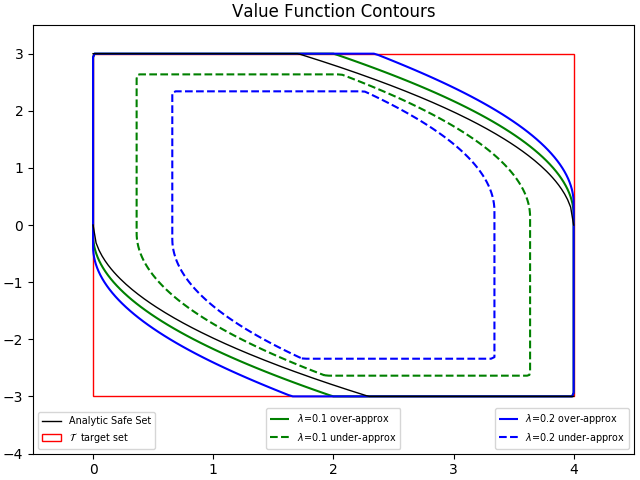
\includegraphics[scale=0.5]{convergence_difflambda.png}
\caption{The analytic reachable set $V$ and target set $\mathcal{T}$ are shown in black and red. The over and under approximated $Z_{\lambda}$ are shown in bold green and dotted green for $\lambda=0.1$; and bold blue and dotted blue line for $\lambda  = 0.2$. This suggests smaller the value of $\lambda$, the better $Z_{\lambda}$ approximates $V$.}
\label{fig:convergence}
\end{figure}

We next compare value iteration and policy iteration with increasing number of discrete actions in Table~\ref{tab:v_vs_p}. In the table we see that as the number of actions increase, there is sharp increase in how long value iteration takes to converge   while the increase is much smaller for policy iteration. However, the total time taken for policy iteration is much larger since there is a significant overhead in building the matrices for value functions. 
\begin{table}
\centering
\caption{Value Iteration vs Policy Iteration}
\label{tab:v_vs_p}
\begin{tabular}{|c| c| c| c|}
\hline
\# actions & VI & \multicolumn{2}{|c|}{Policy Iteration} \\ \cline{3-4}
 &  $T_{total} (Iters)$ & $T_{total}(Iters)$ & $T_{conv}$ \\ \hline
2 & 1.255 (204) & 68.793 (4) & 0.105 \\ \hline
50 &  7.562 (204)&  69.717 (4)& 0.365 \\ \hline
250 & 32.841 (204)&  251.39 (14)& 3.504 \\ \hline
500 & 63.815 (204)&  253.855 (14)& 6.741 \\
\hline
\end{tabular}
\end{table}

Finally, we ran value iteration from different initializations, the signed distance function $Z_0 = l(\cdot)$ and an all zeros $Z_0= 0$. The converged values functions had a norm of $0.000299$ between them, suggesting that MDR converges independent of the initialization. However, running MR with $V_0 = 0$, does not converge to the true value function.

% !TEX root = main_min_disc_dist.tex
\subsection{Pursuit-Evasion Game}

We now consider the pursuit-evasion game described in \cite{Mitchell2005}. In the game player I (the control) tries to avoid being captured by player II (the disturbance) on a two dimensional plane. Each player is modeled as a simple kinematic point object with planar position and heading, fixed linear velocity and controllable angular velocity. Taking player I to be at the origin the states $(x_1, x_2, x_3)$ are the relative position and heading of player II and the dynamics are

\begin{equation}
\begin{split}
&\dot{x_1}= -v_u+v_d \cos x_3 + ux_2\\ 
&\dot{x_2}= v_d \sin x_3 - ux_1\\ 
&\dot{x_3}= d-u
\end{split}
\end{equation}

The state space is over the domain $[-6,20] \times [-10,10] \times [0,2\pi[$ with $\U=[-u_{max},u_{max}]$ and $\D=[-d_{max}, d_{max}]$.

Player I is considered captured when the relative distance (in position) between both players is less than $R>0$, thus the target set is given by

\begin{equation}
\T= \{x| x_1^{2}+x_2^2 < R^2\}
\end{equation}


We first compute the value functions for the MR and MDR on a $41 \times 41 \times 41$ grid, and setting the model parameters to $v_u=v_d=5$, $u_{max}=d_{max}=1$, and $R=5$. This will be referred to as the nominal model $M_n$. A visualization of the zero sub-level set for both $V(x)$ and $Z(x)$ for $\lambda=0.001$ is shown in Fig.~\ref{fig:air3D}.


% \begin{figure}
% 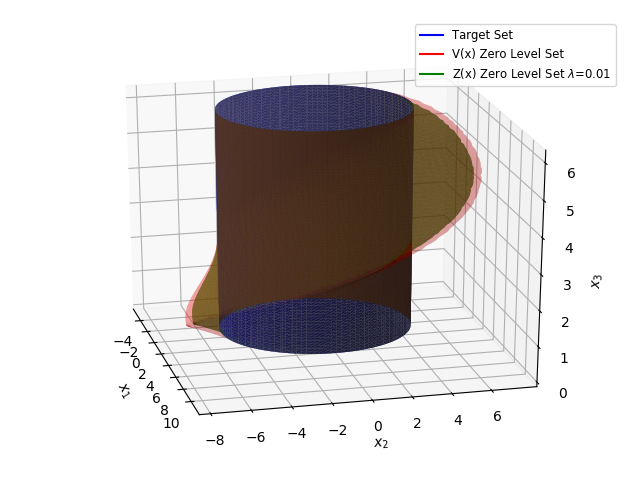
\includegraphics[trim= 2.5cm 0cm 0cm 0.5cm, clip=true,scale=0.65]{air_3D.png}
% \caption{The target set $\mathcal{T}$ is the blue cylinder. The zero sub-level sets of $V$ and $Z$ are in red and green, respectively. The discount rate is $\lambda=0.01$.}
% \label{fig:air3D}
% \end{figure}

\begin{figure*}[h]
    \centering
    \begin{subfigure}[t]{0.3\textwidth}
        \centering
        \includegraphics[trim= 4cm 0cm 0cm 0cm, scale=0.45]{air_3d_v1}
    \end{subfigure}%
    ~ 
    \begin{subfigure}[t]{0.3\textwidth}
        \centering
        \includegraphics[trim= 3cm 0cm 0cm 0cm, clip=true, scale=0.45]{air_3d_v2}
        %\caption{}
    \end{subfigure}
    ~
    \begin{subfigure}[t]{0.3\textwidth}
        \centering
        \includegraphics[trim= 3cm 0cm 0cm 0cm, clip=true, scale=0.45]{air_3d_v3}
        %\caption{}
    \end{subfigure}%
    \caption{The target set $\mathcal{T}$ (blue cylinder), zero sub-level sets of $V$ (red) and $Z$ (green) shown from three different perspectives. The discount rate for $Z$ is $\lambda=0.01$. Note that the zero sub-level set of $Z$ is a subset of the zero sub-level set of $V$.}
    \label{fig:air3D}
\end{figure*}

In the first experiment we compare a multigrid approach to value iteration.  The results are shown in Table~\ref{tab:multigrid_pe}. The experiment and table follows the same structure used for the double integrator model. Similar to the double integrator model, the multigrid approach outperforms value iteration for the pursuit-evasion game.

\begin{table}
\centering
\caption{Pursuit Evasion: Value iteration (VI) with Multigrid}
\begin{tabular}{|c| c| c| c| c| }
\hline
\# nodes & Coarse grid & Fine grid &  Fine grid with WS & Multigrid \\ \hline
$40^3$ & $2.068$ & $29.684$ & $24.320$ & $26.388$ \\ \hline
$80^3$ & $33.166$ & $352.099$ & $317.444$ & $350.610$\\ \hline
\end{tabular}
\label{tab:multigrid_pe}
\end{table}

We now construct two other models by tweaking $M_n$: setting $u_{max}=1.5$, which gives the evader an advantage, we get model $M_e$, and setting $d_{max}=1.5$, which gives the pursuer an advantage,  we get model $M_p$. In the final experiment we look at the impact of initializing value iteration with a solution from a similar model. Just like in the previous benchmark example, this experiment is motivated by Section \ref{sec:model_based}, where now $M_e$ and $M_p$ represent two possible models inferred from the system observations. In this context we have just ``learned" that the evader/pursuer is more maneuverable ($M_e$/$M_p$). We compute both value functions with and without setting the initialization to the solution for $M_n$. Again, we refer to this initialization as a warm start. The results are shown in Table~\ref{tab:ws_pe}.

\begin{table}
\centering
\caption{Pursuit Evasion: Value iteration (VI) with Warm Start (WS)}
\begin{tabular}{|c| c| c| c| c| c|}
\hline
\# nodes & $M_n$ & $M_e$ &  $M_e$ with WS & $M_p$ & $M_p$ with WS \\ \hline
$40^3$ & $35.043$ & $32.242$ & $21.483$ & $26.319$ & $23.366$ \\ \hline
$80^3$ & $439.751$ & $416.965$ & $308.821$ & $300.847$ & $296.568$\\ \hline
\end{tabular}
\label{tab:ws_pe}
\end{table}



\section{Conclusions and Future Work \label{sec:end}}
% !TEX root = main_min_disc_dist.tex

We have presented a novel minimum discounted reward HJ formulation for approximating reachable sets. The main advantage of this new formulation over previous work is that the solution can be obtained as the unique fixed point to a contraction mapping. We also showed how other solutions like policy iteration, and multigrid approaches can be used to yield faster convergence. 

The benefits listed so far, are  within the context of the traditional control paradigm, where we have or assume a fixed model of the system under consideration. However, as learning and data-driven approaches become more powerful and pervasive, perhaps the greatest contribution of this work is that it can lie somewhere in between traditional control and model-free reinforcement learning. The approach is certainly model-based, but because of its agnosticism to initialization it also has the flexibility to incorporate data and build towards solutions iteratively. We foreshadowed how this can be done with temporal difference learning, and in the future we plan on exploring how RL algorithms can be used with this formulation to approximate reachable sets for systems with unknown models or that are high-dimensional. 

\printbibliography

\newpage
% !TEX root = main_min_disc_dist.tex


\begin{IEEEbiography}[{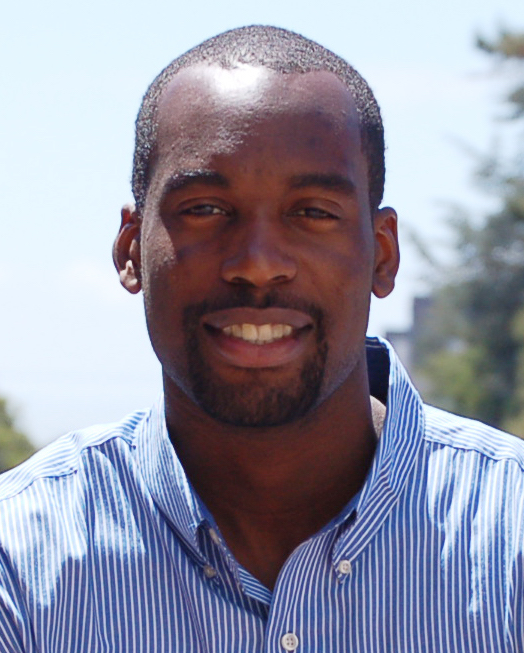
\includegraphics[width=1in,height=1.25in,clip,keepaspectratio]{bio/kene}}]{Anayo K. Akametalu} is a PhD. candidate in Electrical Engineering and Computer Sciences at the University of California, Berkeley. He obtained his B.S. degree in Electrical Engineering from the University of California, Santa Barbara in 2012. His research interests lie at the intersection of control theory and reinforcement learning. He has been funded through the National Science Foundation Bridge to Doctorate Fellowship, UC Berkeley Chancellor's Fellowship, and GEM Fellowship.\end{IEEEbiography}
\vspace{-6cm}
\begin{IEEEbiography}[{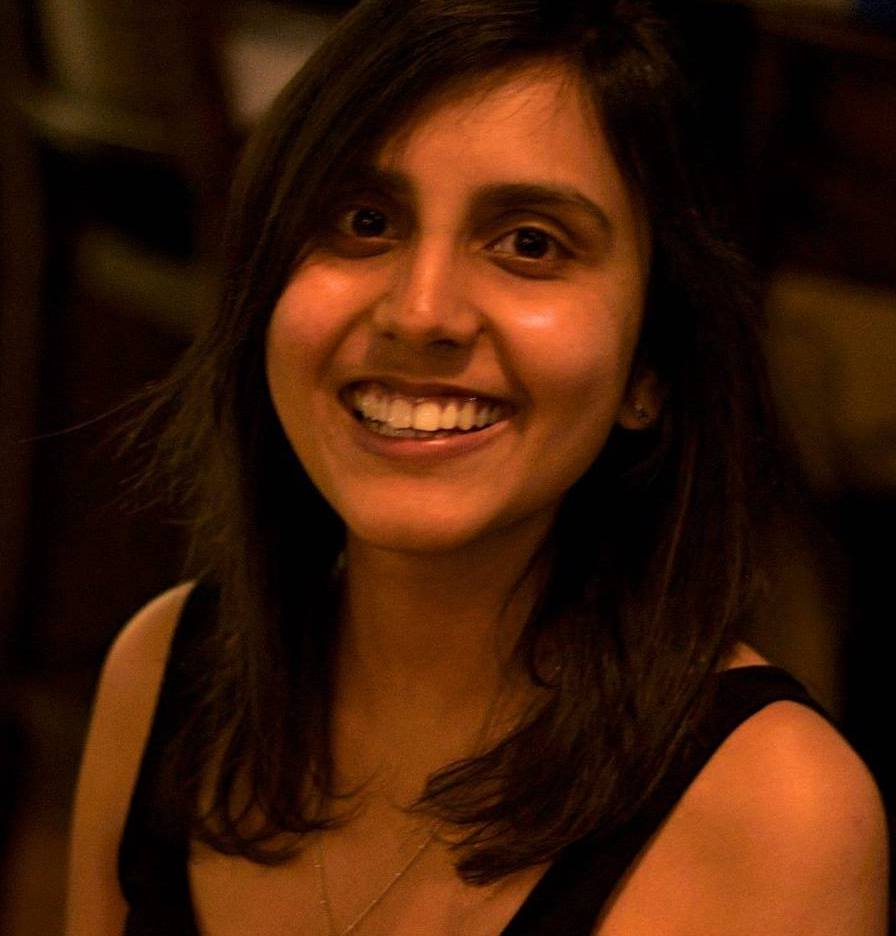
\includegraphics[width=1in,height=1.25in,clip]{bio/shromona}}]{Shromona Ghosh} received her Bachelor in Technology in Electronics and Communication Engineering from National Institute of Technology, Karnataka in 2013. She is currently a PhD candidate at University of California, Berkeley . Her research interests lie in the intersection of Formal Methods, Control Theory and Machine Learning. Specifically, she is looking into developing tools for the formal analysis of systems with learning components. 
\end{IEEEbiography}
\vspace{-6cm}
\begin{IEEEbiography}[{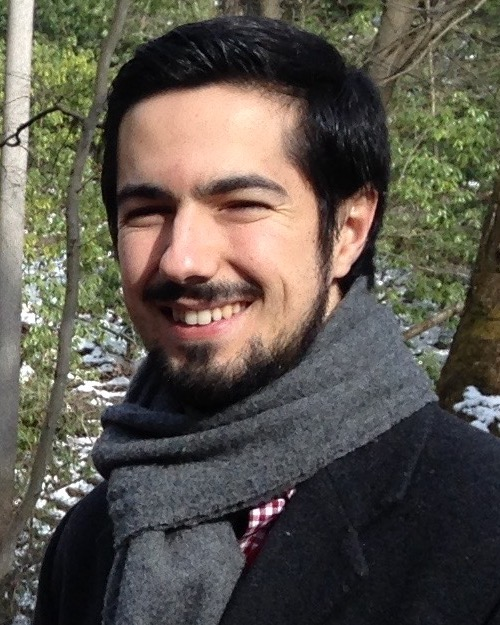
\includegraphics[width=1in,height=1.25in,clip,keepaspectratio]{bio/jaime}}]{Jaime F. Fisac} is a Ph.D. candidate in Electrical Engineering and Computer Sciences at the University of California, Berkeley. He received a B.S./M.S. degree in Electrical Engineering from the Universidad Polit{\'e}cnica de Madrid, Spain, in 2012, and a M.Sc. in Autonomous Vehicle Dynamics and Control from Cranfield University, UK, in 2013. He is a recipient of the ``la~Caixa'' Foundation Fellowship (2013-2015). His research interests lie in control theory, artificial intelligence, and cognitive science, with a focus on safety for robotic and AI systems operating closely with people.
\end{IEEEbiography}
\vspace{-6cm}
\begin{IEEEbiography}[{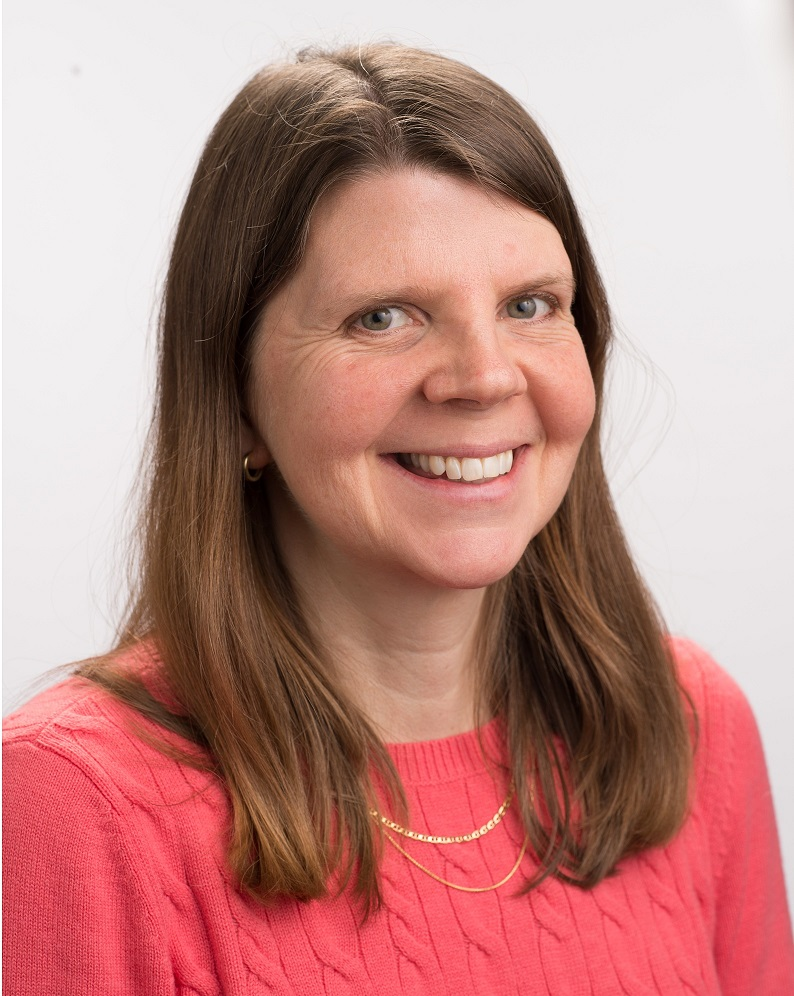
\includegraphics[width=1in,height=1.25in,clip,keepaspectratio]{bio/claire}}]{Claire J. Tomlin} is the Charles A. Desoer Professor of Engineering in Electrical Engineering and Computer Sciences at the University of California, Berkeley. She was an Assistant, Associate, and Full Professor in Aeronautics and Astronautics at Stanford from 1998 to 2007, and in 2005 joined Berkeley. Claire works in the area of control theory and hybrid systems, with applications to air traffic management, UAV systems, energy, robotics, and systems biology. She is a MacArthur Foundation Fellow (2006) and an IEEE Fellow (2010), and in 2010 held the Tage Erlander Professorship of the Swedish Research Council at KTH in Stockholm.
\end{IEEEbiography}


\end{document}
